\documentclass[11pt,a4paper]{article}

% 1. Codificación e Idioma
\usepackage[utf8]{inputenc}
\usepackage[spanish, es-tabla]{babel}

% 2. Paquete de gestión de captiones (añadir esto suele fijar el error)
\usepackage{caption} 
\usepackage{graphicx}
\usepackage{amsmath}
\usepackage{booktabs}
\usepackage[table]{xcolor}
\usepackage{float}
\usepackage{amssymb}
\usepackage{subcaption}
\usepackage{graphicx}
\usepackage{multirow}
\usepackage{tikz}
% 3. Formato y Autores
\usepackage[margin=2.5cm]{geometry}
\usepackage{authblk} 
\usetikzlibrary{babel}
\definecolor{leggreen}{RGB}{85, 170, 85}
\definecolor{legblue}{RGB}{70, 130, 180}
\definecolor{lidarred}{RGB}{200, 80, 80}
\definecolor{background}{RGB}{240, 240, 240}
\definecolor{terrain}{RGB}{139, 69, 19}

\usepackage{hyperref}
\hypersetup{
	colorlinks=true,
	linkcolor=blue,
	urlcolor=blue
}

\usepackage{algorithm}
\usepackage{algpseudocode}
\usepackage{subcaption}
% 4. Bibliografía APA (Cargar al final del preámbulo)

\title{\textbf{Trabajo de Aprendizaje por Refuerzo: Caminante Bípedo}}
\author{
	Jorge Bengoa Pinedo \and
	Bogurad Barañski Barañska
}
\affil{\textbf{Máster TECI - Redes neuronales y aprendizaje estadístico}}
\date{\today}

\begin{document}
	\maketitle
	\section{Introducción}
	En este trabajo se busca abordar mediante aprendizaje por refuerzo el problema del caminante bípedo (\textit{Bipedal Walker}) que consiste en enseñar a un robot en el entorno virtual \textit{Gymnasium} a andar. Para ello, se dispone de los datos de 24 sensores, tal y como se puede ver en la figura \ref{fig:bipedal_walker_obs}, que conforman el espacio de observaciones. A partir de esta información, el robot debe tomar decisiones dinámicas mediante sus 4 actuadores, situados cada uno en una articulación. Estos actuadores se encargan de estabilizar y ejercer movimiento sobre el robot aplicando una velocidad de rotación comprendida entre -1 y 1 $rad/s$.

\begin{figure}[H]
	\centering
	\shorthandoff{>}
	\resizebox{\textwidth}{!}{%
		\begin{tikzpicture}[scale=2, font=\sffamily, every node/.style={rounded corners=2pt, inner sep=3pt}]
			
			% Set a large bounding box to ensure everything fits with ample space
			\draw[white] (-5, -2) rectangle (8, 6.5);
			
			% --- Main Title ---
			\node[anchor=north, font=\LARGE\bfseries, text width=29cm, align=center] at (0.5, 5.5) 
			{Caminante Bípedo de Gymnasium: Espacio de Observaciones (24 Dimensiones)};
			
			% --- The Ground / Terrain ---
			\fill[terrain] (-3.5, 0.2) -- (3.5, 0.2) -- (3.5, -0.5) -- (-3.5, -0.5) -- cycle;
			\draw[ultra thick, brown!80!black] (-3.5, 0.2) -- (3.5, 0.2) node[below right, black] {\textbf{Terreno}};
			
			% --- Lidar / Spatial Sensors (Vars 14-23) ---
			\node[anchor=west, text width=5cm, align=left, fill=lidarred!10, draw=lidarred, thick] (lidartag) at (-1, -1.5)
			{\textbf{Sensores Espaciales (Lidar)} \textbf{(Vars: 14-23)}};
			
			% Simulating 10 beams and connecting them to the hull and tag
			\foreach \x\i in {-2.2/14, -1.8/15, -1.4/16, -1.0/17, -0.6/18, 0.6/19, 1.0/20, 1.4/21, 1.8/22, 2.2/23} {
				\draw[dashed, lidarred, thick] (0, 3) -- (\x, 0.2);
				\draw[->, thin, lidarred] (\x, 0.4) -- (lidartag.north);
			}
			% --- The Hull (Body - Vars 0-3) ---
			\node[anchor=center, 
			draw=black, 
			ultra thick, 
			fill=gray!10, 
			rounded corners=5mm, 
			text width=5.5cm, 
			align=center, 
			inner sep=8pt] (hull) at (0, 3.15) 
			{\textbf{Cuerpo} \\ \color{black}{\textbf{(Vars: 0-3)}}  \\  \color{white}{.} \\  \color{white}{.}};
			% --- Back Leg (Leg 2 - Vars 9-13) ---
			\draw[line width=3mm, legblue] (0.6, 2.7) -- (1.2, 1.5) -- (0.8, 0.2);
			\node[fill=legblue!10, draw=legblue, thick] (hip2callout) at (4.5, 2.9) {Cadera 2 \textbf{(Vars: 9, 10)}};
			\filldraw[white, draw=legblue, ultra thick] (0.6, 2.7) circle (0.15);
			\draw[->, legblue, thick] (hip2callout.west) -- (0.6, 2.7);
			
			\node[fill=legblue!10, draw=legblue, thick] (knee2callout) at (4.5, 1.5) {Rodilla 2 \textbf{(Vars: 11, 12)}};
			\filldraw[white, draw=legblue, ultra thick] (1.2, 1.5) circle (0.15);
			\draw[->, legblue, thick] (knee2callout.west) -- (1.2, 1.5);
			
			\node[fill=legblue!10, draw=legblue, thick] (contact2callout) at (5.0, 0.5) {Contacto con Terreno \textbf{(Var: 13)}};
			\draw[->, legblue, thick] (contact2callout.west) -- (0.8, 0.2);
			
			% --- Front Leg (Leg 1 - Vars 4-8) ---
			\draw[line width=3mm, leggreen] (-0.6, 2.7) -- (-1.2, 1.5) -- (-0.8, 0.2);
			\node[fill=leggreen!10, draw=leggreen, thick] (hip1callout) at (-4.5, 2.9) {Cadera 1 \textbf{(Vars: 4, 5)}};
			\filldraw[white, draw=leggreen, ultra thick] (-0.6, 2.7) circle (0.15);
			\draw[->, leggreen, thick] (hip1callout.east) -- (-0.6, 2.7);
			
			\node[fill=leggreen!10, draw=leggreen, thick] (knee1callout) at (-4.5, 1.5) {Rodilla 1  \textbf{(Vars: 6, 7)}};
			\filldraw[white, draw=leggreen, ultra thick] (-1.2, 1.5) circle (0.15);
			\draw[->, leggreen, thick] (knee1callout.east) -- (-1.2, 1.5);
			
			\node[fill=leggreen!10, draw=leggreen, thick] (contact1callout) at (-5.0, 0.5) {Contacto con Terreno \textbf{(Var: 8)}};
			\draw[->, leggreen, thick] (contact1callout.east) -- (-0.8, 0.2);
			
		
			
			% --- Structured Observation Variables Legend (Right Panel) ---
			\node[anchor=north west, fill=background, draw=black, thick, text width=10cm, inner sep=5pt] (legendpanel) at (8, 6.5) {
				{\Large\bfseries LEYENDA}\vspace{3pt}\hrule\vspace{5pt}
				
				\textbf{Cuerpo (Vars 0-3)}\vspace{2pt}
				\begin{description}
					\item[Var 0:] Ángulo del cuerpo (rad)
					\item[Var 1:] Velocidad angular del cuerpo (rad/s)
					\item[Var 2:] Velocidad horizontal (m/s)
					\item[Var 3:] Velocidad vertical (m/s)
				\end{description}\vspace{5pt}
				
				\textbf{PIERNA 1 (Derecha) (Vars 4-8)}\vspace{2pt}
				\begin{description}
					\item[Var 4:] Ángulo de cadera 1 (rad)
					\item[Var 5:] Vel. angular de cadera 1 (rad/s)
					\item[Var 6:] Ángulo de rodilla 1 (rad)
					\item[Var 7:] Vel. angular de rodilla 1 (rad/s)
					\item[Var 8:] Contacto con el suelo (V/F)
				\end{description}\vspace{5pt}
				
				\textbf{PIERNA 2 (Izquierda) (Vars 9-13)}\vspace{2pt}
				\begin{description}
					\item[Var 9:] Ángulo de cadera 2 (rad)
					\item[Var 10:] Vel. angular de cadera 2 (rad/s)
					\item[Var 11:] Ángulo de rodilla 2 (rad)
					\item[Var 12:] Vel. angular de rodilla 2 (rad/s)
					\item[Var 13:] Contacto con el suelo (V/F)
				\end{description}\vspace{5pt}
				
				\textbf{LIDAR (Vars 14-23)}\vspace{2pt}
				\begin{description}
					\item[Vars 14-23:] Telémetros Lidar \\ 10 mediciones de distancia
				\end{description}
			};
		\end{tikzpicture}%
	}
	\shorthandon{>} 
	\caption{Mapping of the 24-Dimensional Observation Space for the BipedalWalker-v3 Environment}
	\label{fig:bipedal_walker_obs}
\end{figure}

Por tanto, en este trabajo, para la resolución del problema planteado anteriormente se propone abordarlo mediante aprendizaje por refuerzo y, en concreto, utilizando el paradigma de \textit{Soft Actor Critic} descrito en los fundamentos matemáticos a continuación. Este se implementa en \textit{Python} mediante librerías estándar de \textit{stable\_baselines3}, donde primero se realiza una búsqueda exhaustiva de hiperparámetros mediante optimización con \textit{optuna}, para luego entrenar un modelo con los mejores parámetros y ver si el agente aprende a andar.
\newline

Por último, es importante destacar que el objetivo fundamental del aprendizaje por refuerzo en este entorno es que el robot logre cruzar el terreno por completo. Para ello, la función de recompensa se define bajo dos premisas clave: el agente acumula progresivamente hasta 300 puntos si consigue llegar a la meta, pero sufre una fuerte penalización de -100 puntos en el instante en que su cuerpo principal entra en contacto con el suelo. Además, se aplica un castigo por el uso excesivo de torque en los articulaciones. Esta limitación tiene como propósito desincentivar los movimientos erráticos y asegurar que la marcha aprendida sea transferible a casos reales, donde la saturación de los motores tiene un alto coste físico.

\section{Fundamentos matemáticos}
	\section{Procesos de decisión de Markov}
	
	La siguiente sección se ha escrito de acuerdo a \cite{barto2021reinforcement}. 
	
	Los procesos de decisión de Markov (MDP) sirven para modelar el aprendizaje mediante interacción para conseguir un objetivo. Los MDP comprenden dos elementos:
	
	\begin{itemize}
		\item Agente: es el que aprende y toma decisiones. 
		\item Entorno: comprende todo lo que es externo al agente e interactúa con el agente.
	\end{itemize}
	 
	 Cuando el agente toma una decisión, el entorno presenta una nueva situación al agente. Además, le entrega una recompensa. Mediante sus acciones, el agente busca maximizar la recompensa obtenida a lo largo del tiempo. La figura \ref{fig:mdp} refleja estas interacciones.
	 
	 \begin{figure}[H]
	 	\centering
	 	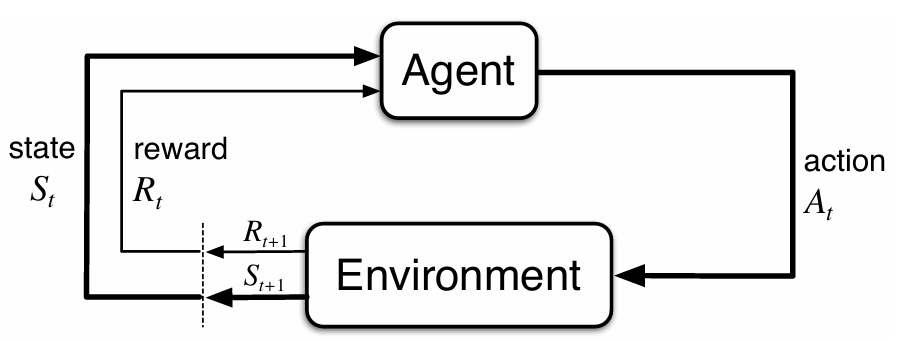
\includegraphics[width=0.7\linewidth]{figuras/mdp.png}
	 	\caption{Interacción entre agente y entorno a través de un proceso de decisión de Markov.}
	 	\label{fig:mdp}
	 \end{figure}
	 
	Sean $\mathcal{S}$, $\mathcal{A}$ y $\mathcal{R}$ los conjuntos de estados, acciones y recompensas, respectivamente, entonces:
	
	\begin{align}
	& p: \mathcal{S} \times \mathcal{R} \times \mathcal{S} \times \mathcal{A} \to [0,1] \nonumber \\
	& p(s', r \mid s, a) = \Pr{S_t = s', R_t = r \mid S_{t-1} = s, A_{t-1} = a} \nonumber \\
	& \sum_{s' \in \mathcal{S}} \sum_{r \in \mathcal{R}} p(s', r \mid s, a) = 1, \quad \forall s \in \mathcal{S}, a \in \mathcal{A}(s) 
	\end{align}
	
	Donde $s, s' \in \mathcal{S}$, $r \in R$, $a \in A$. A partir de la ecuación anterior, se puede calcular la probabilidad marginal del siguiente estado:
	
	\begin{align}
	& p: \mathcal{S} \times \mathcal{S} \times \mathcal{A} \to [0,1] \nonumber \\
	& p(s' \mid s, a) = \Pr\{S_t = s' \mid S_{t-1} = s, A_{t-1} = a\} = \sum_{r \in \mathcal{R}} p(s', r \mid s, a) 
	\end{align}
	
	Y la recompensa esperada: 
	\begin{align}
		& r: \mathcal{S} \times \mathcal{A} \to \mathbb{R} \nonumber \\
		& r(s, a) = \mathbb{E}[R_t \mid S_{t-1} = s, A_{t-1} = a] = \sum_{r \in \mathcal{R}} r  \cdot p(r \mid s, a) = \sum_{r \in \mathcal{R}} r \sum_{s' \in \mathcal{S}} p(s', r \mid s, a)
	\end{align}
	
	\subsection{Aprendizajes episódico y continuo}
	El objetivo del agente es maximizar la recompensa esperada en el largo plazo. Esto implica conocer cómo una acción presente repercute en los sucesivos pasos temporales. Según se tenga un estado final o no, se distingue entre:
	
	\begin{itemize}
		\item Aprendizaje episódico: cada episodio tiene una duración $T$ finita, que no tiene por qué ser fija (p.ej. partidas de ajedrez). La recompensa esperada a maximizar se podría escribir como:
		
		\begin{equation}
		G_t = R_{t+1} + R_{t+2} + \cdots + R_T
		\end{equation}
		
		\item Aprendizaje continuo: las interacciones agente-entorno no tienen un fin o este es muy lejano (p.ej. un robot \textit{pick and place}). En tal caso, la definición anterior podría tomar el valor $\infty$. Para evitarlo, se define la recompensa descontada:
		
		\begin{equation}
		G_t = \sum_{k=0}^{\infty} \gamma^k R_{t+k+1} = R_{t+1} + \gamma \sum_{k=1}^\infty \gamma^{k-1} R_{t+k+1} = R_{t+1} + \gamma G_{t+1}
		\end{equation}
		
		Donde $\gamma$ es el factor de descuento. Si $\gamma < 1$, el sumatorio converge a un valor finito. Cuanto mayor sea el valor de $\gamma$, mayor visión a futuro tendrá el agente.
	\end{itemize}
	
	Se puede adoptar una notación común a ambos problemas:
	
	\begin{equation}
	G_t = \sum_{k=t+1}^{T} \gamma^{k-t-1} R_{k}
	\end{equation}
	
	Donde las condiciones $\gamma=1$ y $T=\infty$ son mutuamente excluyentes y representan los casos episódico y continuo de forma excluyente.
	
	\subsection{Políticas y funciones de valor}
	Una política define la probabilidad de que el agente tome una determinada acción dado un estado. Se denotará por $\pi(a \mid s)$. 
	
	Por otro lado, las funciones de valor pueden ser:
	
	\begin{itemize}
		\item Funciones de estado-valor: determinan cómo de bueno es que el agente esté en un determinado estado:
		
		\begin{equation}
		v_\pi(s) = \mathbb{E}_\pi[G_t \mid S_t = s] = \mathbb{E}_\pi \left[ \sum_{k=0}^\infty \gamma^k R_{t+k+1} \;\middle|\; S_t = s \right], \forall s \in \mathcal{S}
		\end{equation}
		
		La función estado-valor óptima es:
		
		\begin{equation}
		v_{*}(s) = \max_{\pi} v_\pi(s), \forall s \in \mathcal{S}
		\end{equation}
		
		\item Funciones de acción-valor: determinan cómo de bueno es que el agente tome una dterminada acción dado un estado:
		
		\begin{equation}
		q_\pi(s, a) = \mathbb{E}_\pi[G_t \mid S_t = s, A_t = a] = \mathbb{E}_\pi \left[ \sum_{k=0}^\infty \gamma^k R_{t+k+1} \;\middle|\; S_t = s, A_t = a \right]
		\end{equation}
		
		Se dice que una política es óptima si $v_*(s) \ge v_\pi(s), \forall s \in S, \forall \pi$. La función acción-valor óptima es:
		
		\begin{equation}
		q_{*}(s,a) = \max_{\pi} q_\pi(s,a) = \mathbb{E}\left[ R_{t+1} + \gamma v_{*}(S_{t+1}) \mid S_t = t, A_t = a \right], \forall s \in \mathcal{S}, a \in \mathcal{A}
		\end{equation}
	\end{itemize}
	
	A partir de las expresiones anteriores se deduce la ecuación de expectativa de Bellman sobre la función estado-valor:
	
	\begin{align}
	v_\pi(s) &= \mathbb{E}_\pi[G_t \mid S_t = s] = \mathbb{E}_\pi[R_{t+1} + \gamma G_{t+1} \mid S_t = s] \nonumber \\
	&=\sum_{a \in \mathcal{A}} \pi(a \mid s) \mathbb{E}_\pi[R_{t+1} + \gamma G_{t+1} \mid S_t = s, A_t = a] && \text{(Ley de la probabilidad total)} \nonumber \\
	&=\sum_{a \in \mathcal{A}} \pi(a \mid s) \sum_{s' \in \mathcal{S}} \sum_{r \in \mathcal{R}} p(s', r \mid s, a) \cdot \nonumber \\
	&\qquad\mathbb{E}_\pi[R_{t+1} + \gamma G_{t+1} \mid S_t = s, A_t = a, S_{t+1} = s', R_{t+1} = r] && \text{(Ley de la probabilidad total)} \nonumber \\
	&=\sum_{a \in \mathcal{A}} \pi(a \mid s) \sum_{s',r} p(s', r \mid s, a) \mathbb{E}_\pi[R_{t+1} + \gamma G_{t+1} \mid S_{t+1} = s'] && \text{(Propiedad Markoviana)} \nonumber \\
	&=\sum_{a \in \mathcal{A}} \pi(a \mid s) \sum_{s',r} p(s', r \mid s, a) \mathbb{E}_\pi[r+ \gamma G_{t+1} \mid S_{t+1} = s'] && \text{(Propiedad Markoviana)} \nonumber\\
	&=\sum_{a \in \mathcal{A}} \pi(a \mid s) \sum_{s',r} p(s', r \mid s, a) \left[ r + \gamma \mathbb{E}_\pi[G_{t+1} \mid S_{t+1} = s'] \right] \nonumber \\
	&=\sum_{a \in \mathcal{A}} \pi(a \mid s) \sum_{s',r} p(s', r \mid s, a) \left[ r + \gamma v_{\pi}(s') \right]
	\end{align}
	
	Análogamente, se puede obtener la ecuación de optimalidad de Bellman sobre la función estado-valor (nótese que la función estado-valor óptima corresponde con seguir la política óptima partiendo de la acción que maximiza la recompensa):
	
	\begin{align}
	v_{*}(s) &= \max_{a \in \mathcal{A}(s)} q_{\pi^*}(s, a) \nonumber \\
	&= \max_a \mathbb{E}_{\pi^*} [G_t \mid S_t = s, A_t = a] \nonumber \\
	&= \max_a \mathbb{E}_{\pi^*} [R_{t+1} + \gamma G_{t+1} \mid S_t = s, A_t = a] \nonumber \\
	&= \max_a \mathbb{E} [R_{t+1} + \gamma v_{*}(S_{t+1}) \mid S_t = s, A_t = a] \nonumber \\
	&= \max_{a} \sum_{s', r} p(s', r \mid s, a) \left[ r + \gamma v_{*}(s') \right]
	\end{align}
	
	Las mismas ecuaciones de Bellman se pueden deducir para la función acción-valor:
	
	\begin{align}
	& q_{\pi}(s,a) = \mathbb{E}_\pi[R_{t+1} + \gamma G_{t+1} \mid S_t = s, A_t = a] = \sum_{s',r} p(s', r \mid s, a) \left[ r + \gamma v_{\pi}(s') \right] \\
	& q_*(s,a) = \mathbb{E}_\pi[R_{t+1} + \gamma \max_{a'} q_*(S_{t+1}, a') \mid S_t = s, A_t = a] = \sum_{s',r} p(s', r \mid s, a) \left[ r + \gamma \max_{a'} q_*(s',a') \right]
	\end{align}
	
	Conocido el valor de $v_*(s)$, bastaría con mirar el siguiente estado con ese valor esperado y seleccionar la acción que conduce a dicho estado. Como la información a largo plazo está codificada en la propia función estado-valor óptima, moverse de forma codiciosa (\textit{greedy}), es decir, mirando solo al siguiente instante, ya implica tener en cuenta el futuro. Conocido $q_*(s,a)$, el problema es aún más fácil ya que no haría falta conocer que acción conduce al siguiente estado. Tan solo habría que seleccionar la acción cuyo valor sea óptimo. \\
	
	Lógicamente, resolver las ecuaciones de Bellman puede no ser factible debido a que se necesitaría memoria y potencia computacional infinitas. Por lo tanto, se usan aproximaciones de las funciones estado-valor y acción-valor. Aunque los resultados son subóptimos, suelen funcionar razonablemente bien. Las políticas óptimas resultantes tienden a poner más esfuerzo en aprender de los estados que ocurren frecuente y menos esfuerzo en los menos habituales.
	
	\section{Aprendizaje por diferencias temporales}
	Idealmente, la política óptima se deriva de las ecuaciones de optimalidad de Bellman. Sin embargo, su resolución no es trivial, por lo que aparecen distintos esquemas para aproximar $v_*(s)$ y $q_*(s,a)$:
	
	\begin{itemize}
		\item Métodos de Monte-Carlo: no requieren un modelo del entorno. Las funciones de valor aproximadas se actualizan al final de cada episodio, estimando la esperanza a partir de una muestra.
		\item Programación dinámica: no requiere esperar al final de cada episodio para su actualización (permiten aprendizaje continuo), ya que calcula la esperanza exacta de las funciones de valor al suponer conocido un modelo del entorno.
		\item Diferencias temporales: aproximan las funciones valor sin necesidad de esperar el final de cada episodio ni de un modelo del entorno.
	\end{itemize}
	
	El enfoque de diferencias temporales combina las ventajas de los métodos de Monte-Carlo y la programación dinámica, haciéndolo flexible ante diversas situaciones.
	
	\subsection{Predicción TD}
	El problema de predicción consiste en estimar la función de valor $v_\pi$ a partir de la experiencia siguiendo una política $\pi$. El método TD(0) es el más simple de todos. Actualiza su estimación en el instante $t+1$ utilizando la recompensa inmediata observada y la estimación de $v_\pi$ en el siguiente estado:
	
	\begin{equation}
	V(S_t) \leftarrow V(S_t) + \alpha \left[ R_{t+1} + \gamma V(S_{t+1}) - V(S_t) \right] = V(S_t) + \alpha \delta_t
	\end{equation}
	
	Donde $\alpha \in (0, 1]$ es la tasa de aprendizaje y $\delta_t = R_{t+1} + \gamma V(S_{t+1}) - V(S_t)$ es el error TD. Este último mide la diferencia entre la estimación actual, $V(S_t)$, y una estimación mejorada respaldada por la experiencia, $R_{t+1} + \gamma V(S_{t+1})$.
	
	Otra ventaja de los métodos TD frente a Monte-Carlo es que son más robustos ante acciones arbitrarias de exploración. En los métodos de Monte-Carlo, este tipo de acciones podría distorsionar el valor de la esperanza, por lo que habría que descartar la iteración. Los métodos TD, por contra, aprenden de cada transición. \\
	
	Los métodos TD convergen a la media de $v_\pi$ si se sigue una política fija, $\pi$, y $\alpha$ es constante y suficientemente pequeño. La probabilidad de convergencia es 1 si $\alpha$ se reduce gradualmente, cumpliendo ciertas condiciones. No obstante, muchas de las pruebas de convergencia solo aplican al caso tabular.\\
	
	Respecto a la velocidad de convergencia, los métodos TD convergen más rápido que Monte-Carlo de forma práctica, aunque no haya una demostración matemática. Esto ocurre para el formato online y batch (acumulando el error TD sobre todas las muestras disponibles antes de actualizar).
	
	\subsection{Control TD}
	El problema de control consiste en estimar $q_\pi(s,a)$. Por lo tanto, la actualización depende de los pares estado-acción. Existen distintas variantes de los métodos TD para este tipo de problemas:
	
	\begin{itemize}
		\item SARSA: es el caso más simple:
		
		\begin{equation}
		Q(S_t, A_t) \leftarrow Q(S_t, A_t) + \alpha \left[ R_{t+1} + \gamma Q(S_{t+1}, A_{t+1}) - Q(S_t, A_t) \right]
		\end{equation}
		
		Es un algoritmo on-policy (la misma política seguida para la transición de estados es la que se actualiza) en el que continuamente se estima $q_\pi$ a la vez que se va modificando la política $\pi$ para que tienda a la codicia. Se empieza con una política que permite la exploración con una cierta probabilidad. Cada vez se favorece más las decisiones de explotación (seleccionar las recompensas que maximizan las acciones) en contra de dicha exploración.
		
		\item Q-learning: es un algoritmo off-policy que converge a $q_*$:
		
		\begin{equation}
		Q(S_t, A_t) \leftarrow Q(S_t, A_t) + \alpha \left[ R_{t+1} + \gamma \max_a Q(S_{t+1}, a) - Q(S_t, A_t) \right]
		\end{equation}
		
		La política de comportamiento para moverse por los estados puede elegirse libremente, lo que favorece la exploración. A medida que se van observando los estados, la política objetivo aprende a seleccionar la acción que maximiza la recompensa. Una ventaja de los métodos off-policy es que no importa cómo se han generado las muestras a la hora de actualizar la política objetivo, ya que ambas están desagregadas. Los métodos on-policy se actualizan de acuerdo a los estados explorados según la política actual. Es decir, no pueden reutilizar datos pasados porque fueron generados con una política diferente. 
		
		\item Expected SARSA:
		
		\begin{align}
		Q(S_t, A_t) &\leftarrow Q(S_t, A_t) + \alpha \left[ R_{t+1} + \gamma \mathbb{E}_\pi \left[ Q(S_{t+1}, A_{t+1}) \mid S_{t+1} \right] - Q(S_t, A_t) \right] \nonumber \\
		&= Q(S_t, A_t) + \alpha \left[ R_{t+1} + \gamma \sum_a \pi(a|S_{t+1}) Q(S_{t+1}, a) - Q(S_t, A_t) \right]
		\end{align}
		
		En vez de evaluar el siguiente par estado-acción, usa su valor esperado. La política objetivo $\pi$ puede ser la misma que la de comportamiento (on-policy) o distinta (off-policy). Reduce la varianza asociada a elegir una única acción $A_{t+1}$ de forma aleatoria a cambio de un mayor coste computacional.
		
		\item Double-Q-learning: utiliza dos funciones de acción-valor para desacoplar la acción de la evaluación:
		
		\begin{align}
		& Q_1(S_t, A_t) \leftarrow Q_1(S_t, A_t) + \alpha \left[ R_{t+1} + \gamma Q_2(S_{t+1}, \arg\max_a Q_1(S_{t+1}, a)) - Q_1(S_t, A_t) \right] \\
		& Q_2(S_t, A_t) \leftarrow Q_2(S_t, A_t) + \alpha \left[ R_{t+1} + \gamma Q_1(S_{t+1}, \arg\max_a Q_2(S_{t+1}, a)) - Q_2(S_t, A_t) \right]
		\end{align}
		
		El Q-learning es optimista cuando las recompensas son ruidosas. Intuitivamente, se puede imaginar la situación en que los valores reales $q(s,a)$ son todos cero, pero sus estimaciones $Q(s,a)$ presentan incertidumbre. El máximo de los valores reales es cero, mientras que el máximo estimado es positivo. Esto se conoce como sesgo de maximización. \\
		
		El double-Q-learning aborda este problema calculando simultáneamente dos funciones acción-valor: $Q_1(s,a)$ y $Q_2(s,a)$. Pero en cada iteración se actualiza solamente una de ellas a partir de la evaluación según la otra. Si una recompensa es ruidosa en torno a cero, será raro que tome valores positivos constantemente. Por ejemplo, para la primera muestra se actualiza $Q_1$, que ve una recompensa muy alta. Si se usara Q-learning, otros pares estado-acción aumentarían su valor solamente por la expectativa de volver a repetir la jugada. Sin embargo, $Q_2$ evalúa el par estado-acción sin haber visto tal recompensa. Su percepción será que dicho par estado-acción no tiene tanto valor. Este proceso se repite actualizando arbitrariamente cada función.
		
	\end{itemize}
	\subsection{Optimización de cajas negras costosas}
	Debido al alto costo computacional del entrenamiento en aprendizaje por refuerzo, es fundamental optimizar la búsqueda de hiperparámetros reduciendo las evaluaciones de la función objetivo (en este trabajo, en entrenamientos de 50,000 épocas). En lugar de emplear un barrido por fuerza bruta, se utiliza una estrategia de optimización basada en Estimadores de Parzen en Estructura de Árbol (TPE) \cite{NIPS2011_86e8f7ab}, la cual permite un muestreo de parámetros más eficiente.
	\newline
	
	En este artículo se emplea un algoritmo de Optimización Global Secuencial Basada en Modelos (SMBO), detallado en el Algoritmo \ref{alg:SMBO}. De manera intuitiva, este procedimiento busca minimizar las evaluaciones de la función de coste $f(x)$ mediante la construcción de modelos bayesianos a partir de un historial de observaciones $\mathcal{H}$, el cual almacena las tuplas de parámetros evaluados y sus respectivos resultados. Para ello, se ajusta un modelo simplificado $M_t$ a la muestra $\mathcal{H}$ utilizando un estimador. En este trabajo se utiliza TPE, aunque el proceso también admite distribuciones normales conjugadas. Dado que optimizar un criterio de selección o función de adquisición $S(x, M_{t-1})$ es computacionalmente mucho más sencillo que evaluar la caja negra original, el algoritmo utiliza este modelo para identificar puntos \(x^*\) que ofrezcan una mayor probabilidad de mejorar el rendimiento en la función objetivo reduciendo así el número de llamadas necesarias a la función objetivo.
	\begin{algorithm}[H]
		\caption{Pseudo-código SMBO.}
		\label{alg:SMBO}
		\begin{algorithmic}[1]
			\State \textbf{SMBO}($f, M_0, T, S$)
			\State $\mathcal{H} \leftarrow \emptyset$,
			\For{$t \leftarrow 1$ \textbf{to} $T$,}
			\State $x^* \leftarrow \text{argmax}_x S(x, M_{t-1})$,
			\State Evaluate $f(x^*)$, \hfill $\triangleright$ Expensive step
			\State $\mathcal{H} \leftarrow \mathcal{H} \cup (x^*, f(x^*))$,
			\State Fit a new model $M_t$ to $\mathcal{H}$.
			\EndFor
			\State \textbf{return} $\mathcal{H}$
		\end{algorithmic}
	\end{algorithm}
	
	
	Para el estimador \(S(x, M_{t-1})\) se utiliza el estimador de Mejora Esperada (EI) definido para un problema de maximización como:
	\begin{equation}
		EI_{y^*}(x)=\int_{-\infty}^{\infty} \max(y-y^*,0)\cdot p_{M}(y|x) dy
	\end{equation}
	donde \(y^*\) representa una cota inferior a partir de la cual aceptar un punto como válido dentro del modelo y \(p_{M}(y|x)\) representa la distribución a posteriori del modelo simplificado de \(f(x)\) construida a partir de las distribuciones de verosimilitud de los datos mediante TPE.
	\newline
	
	La justificación detrás del uso de TPEs y no modelos gausianos reside en que cuando se ajustan hiperparámetros en modelos por refuerzo o basados en redes el espacio de configuración es jerárquico y hasta cierto punto categórico. En TPE se modelan la probabilidad $p(x|y)$ mediante la partición del espacio muestral $\mathcal{H}$ en dos densidades diferenciadas según una cota de rendimiento $y^*$:
	
	\begin{equation}
		p(x|y) = 
		\begin{cases} 
			\ell(x) & \text{si } y > y^* \\ g(x) & \text{si } y \leq y^*
		 \end{cases}
		 \label{eq:22}
	\end{equation}
	
	En esta formulación de maximización, $\ell(x)$ representa la densidad de los puntos con mejores resultados (superiores a $y^*$) y $g(x)$ la del resto de observaciones. El umbral $y^*$ se establece como un cuantil $\gamma$ del historial, de forma que $p(y > y^*) = \gamma$. 
	\newline
	
	Al aplicar la regla de Bayes, se demuestra que la Mejora Esperada es proporcional a la relación entre estas densidades:
	
	\begin{equation}
		EI_{y^*}(x) \propto \left( \gamma + \frac{g(x)}{\ell(x)}(1 - \gamma) \right)^{-1}
	\end{equation}
	
	Esta expresión indica que para maximizar la mejora se deben buscar puntos con una alta probabilidad según $\ell(x)$ y baja probabilidad según $g(x)$. Ambas funciones, se construyen dinámicamente en función de la variable estudiada tal y como se describe a continuación:
	\begin{itemize}
		\item \textbf{Variables continuas:} Se utilizan mezclas de Gausianas equiprobables centradas en cada uno de los valores experimentales obtenidos, donde la desviación típica es la mayor de las distancias a sus vecinos. En este caso, las funciones \(\ell(x)\) y $g(x)$ se construyen teniendo en cuenta sólo los puntos que cumplen la inecuación \ref{eq:22}. Por tanto, teniendo en cuenta la existencia de una distribución a priori y un parámetro de regularización $\omega$ la expresión de estas funciones es:
		\begin{equation}
				g(x)\text{ o }  \ell(x)= w \cdot P_{priori}(x) + \frac{1-w}{K} \sum_{i=1}^{K} \mathcal{N}(x | x^{(i)}, \sigma_i^2)
		\end{equation}
		\item \textbf{Variables discretas:} Suponiendo la distribución a priori como un vector de \(N\) probabilidades \(p_i\), la distribución del vector a posteriori es proporcional a \(N\cdot p_i + C_i\) con \(C_i\) el número de apariciones de la variable \(i\) en el espacio muestral.
	\end{itemize}
	
	
	
	Así, el algoritmo genera candidatos según $\ell(x)$ y selecciona aquel que maximiza la relación $\ell(x)/g(x)$, optimizando la búsqueda de manera eficiente.
	\newline
	
	
	Otro paso adicional que se puede tomar dentro de la optimización de cajas negras costosas como es en el caso del aprendizaje por refuerzo es que, como se obtienen valores intermedios de las evaluaciones, se puede asumir que si un ensayo no es competitivo en sus etapas iniciales, es preferible detener su ejecución para ahorrar recursos (aunque esta suposición es debatible tal y como se verá en los resultados). Para ello, se implementa la Regla de Parada de la Mediana descrita en \cite{46180}, la cual cancela un ensayo en el paso $s$ si su mejor valor objetivo es estrictamente peor que la mediana de los promedios acumulados de todos los experimentos completados hasta ese mismo punto.
	
	\section{Metodología}
	Para abordar los pasos de entrenamiento, evaluación y análisis del agente de aprendizaje por refuerzo en el entorno del caminante bípedo se ha diseñado una metodología secuencial dividida en cuatro fases.
	
	\subsection{Optimización de Hiperparámetros (Finetuning)}
	Para maximizar el rendimiento del algoritmo Soft Actor-Critic (SAC), se implementó un proceso de búsqueda automatizada de hiperparámetros utilizando la librería \textit{Optuna}.
	\newline
	
	El primer paso dentro de la optimización consiste en definir el espacio de búsqueda en el cual se definen los siguientes valores a analizar de los hiperparámetros:
	\begin{itemize}
		\item \textbf{Tasa de aprendizaje:} Variable continua en escala logarítmica en el intervalo \([ 10^{-5}, 10^{-2}]\).
		\item \textbf{Tamaño del lote de entrenamiento (\textit{Batch}):} Variable discreta con valores \((128, 256, 512)\).
		\item \textbf{Arquitectura de la red neuronal:} Variable discreta con valores \((128, 256, 300, 400)\) neuronas por capa.
		\item \textbf{Factor de suavizado $\tau$:} Variable continua en escala logarítmica en el intervalo \([0.001,0.05]\).
		\item \textbf{Factor de descuento $\gamma$:} Variable discreta con valores \((0.98, 0.99, 0.995, 0.999)\).
	\end{itemize}
	
	El segundo paso de la optimización consiste en implementar una poda mediante mediana donde evaluando periódicamente cada 10,000 pasos se evalúa el rendimiento de los modelos en la fase de entrenamiento para ver si fuera necesario interrumpir el entrenamiento de manera prematura para así reducir la carga computacional.
	\newline
	
	Por último, en la fase de ejecución se realizan 100 evaluaciones a la caja negra costosa mediante el optimizador bayesiano de \textit{Optuna} donde cada una de las evaluaciones consistía de un entrenamiento de 50,000 pasos de simulación. Para cada iteración se registraban las métricas de rendimiento y la configuración utilizada en cada caso. 


	\subsection{Entrenamiento del Modelo Final}
	Tras analizar los resultados de la fase de optimización, se procede a entrenar el agente definitivo utilizando la configuración de hiperparámetros que dan la mejor recompensa tal como se muestra en la tabla \ref{tab:hiperparametros_finales}:
	
	\begin{table}[H]
		\centering
		\begin{tabular}{ll}
			\hline
			\textbf{Hiperparámetro} & \textbf{Valor Seleccionado} \\ \hline
			Algoritmo & Soft Actor-Critic (SAC) \\
			Arquitectura de Red (net\_arch) & [256, 256] \\
			Tasa de Aprendizaje (Learning Rate) & $1.965 \times 10^{-4}$ \\
			Tamaño de Lote (Batch Size) & 512 \\
			Factor de Descuento ($\gamma$) & 0.995 \\
			Coeficiente de Suavizado ($\tau$) & 0.0388 \\
			Coeficiente de Entropía ($\alpha$) & Automático (\textit{auto}) \\
			Buffer de Memoria & 300,000 pasos \\ \hline
		\end{tabular}
		\caption{Configuración de hiperparámetros óptimos seleccionada para el entrenamiento final.}
		\label{tab:hiperparametros_finales}
	\end{table}
	
	Durante la simulación de 500,000 pasos, se establecieron dos rutinas para el registro de datos. Por un lado, se evalúa el rendimiento cada 1,000 pasos para guardar siempre el mejor modelo histórico. Por otro, se guardan copias del modelo cada 5,000 pasos con el objetivo de documentar y analizar la evolución cronológica del entrenamiento.

	\subsection{Simulación y Registro Visual}
	Para observar cómo aprende a moverse el agente, se creó un script que graba vídeos automáticamente a partir de los modelos guardados durante el entrenamiento.
	
	\begin{itemize}
		\item \textbf{Modificación del entorno:} Se programó un \textit{Wrapper} personalizado que captura cada fotograma del simulador, amplía la imagen y añade una banda de texto en la parte inferior. De este modo, en el vídeo siempre se indica en qué paso del entrenamiento se encuentra el modelo evaluado.
		\item \textbf{Creación del vídeo resumen:} Se ejecutó una simulación de 500 pasos para cada uno de los 60 modelos almacenados. Después, todos estos clips se unieron utilizando FFmpeg sin perder calidad. El resultado es un único vídeo que muestra de forma continua cómo el robot pasa de moverse al azar en los primeros intentos a caminar correctamente.
	\end{itemize}
	
	\subsection{Análisis Estadístico y Visualización}
	La última fase de la metodología consistió en el procesamiento de los registros crudos para evaluar la convergencia y estabilidad del algoritmo matemático tal y como se puede ver en las gráficas de los resultados.

	\section{Resultados}
	
	El primer resultado a mostrar es el del coste computacional del algoritmo que tal y cómo se puede ver en la tabla \ref{tab:tiempos_metodologia} es elevado pese a que se ha entrenado en una GPU potente como lo es una NVDIA 4070.
	\begin{table}[H]
		\centering
		\begin{tabular}{lc}
			\hline
			\textbf{Fase de Trabajo} &  \textbf{Tiempo Total} \\ \hline
			Optimización (Optuna) & 8h 22min \\
			Entrenamiento Final (SAC) &  2h 26min \\
			Generación de Timelapse & 35min \\ \hline
			\textbf{Total Acumulado} &  \textbf{11h 23min} \\ \hline
		\end{tabular}
		\caption{Cronología y Coste Computacional del Proceso de Entrenamiento}
		\label{tab:tiempos_metodologia}
	\end{table}
	
	La figura \ref{fig:analisis_optuna_completo} se detalla el impacto de los hiperparámetros sobre la recompensa obtenida. Como se observa, en la gran mayoría de los ensayos el agente fue incapaz de avanzar y terminó cayendo rápidamente. Sin embargo, en todas las gráficas destaca un claro outlier positivo, el cual corresponde a la configuración finalmente seleccionada. Este modelo logra mantener al caminante estable durante una mayor cantidad de pasos, convirtiéndose en el mejor candidato al ser el único que mostró signos reales de aprendizaje en 50.000 pasos.
	\newline
	
	Respecto al resto de combinaciones, resulta complejo extraer conclusiones definitivas. Como se analizará más adelante, el límite de 50.000 pasos fijado para la fase de optimización es un horizonte temporal bastante restrictivo. Los algoritmos de aprendizaje por refuerzo suelen presentar una convergencia no lineal. Pues tal como se verá estos algoritmos atraviesan largas fases iniciales donde la recompensa oscila sin mejoras evidentes, seguidas de un salto abrupto en el rendimiento una vez que el agente asimila aprende a realizar la tarea donde ya se mantendrá estable.
	
	\begin{figure}[H]
		\centering
		% Subfigura (a)
		\begin{subfigure}[b]{0.48\textwidth}
			\centering
			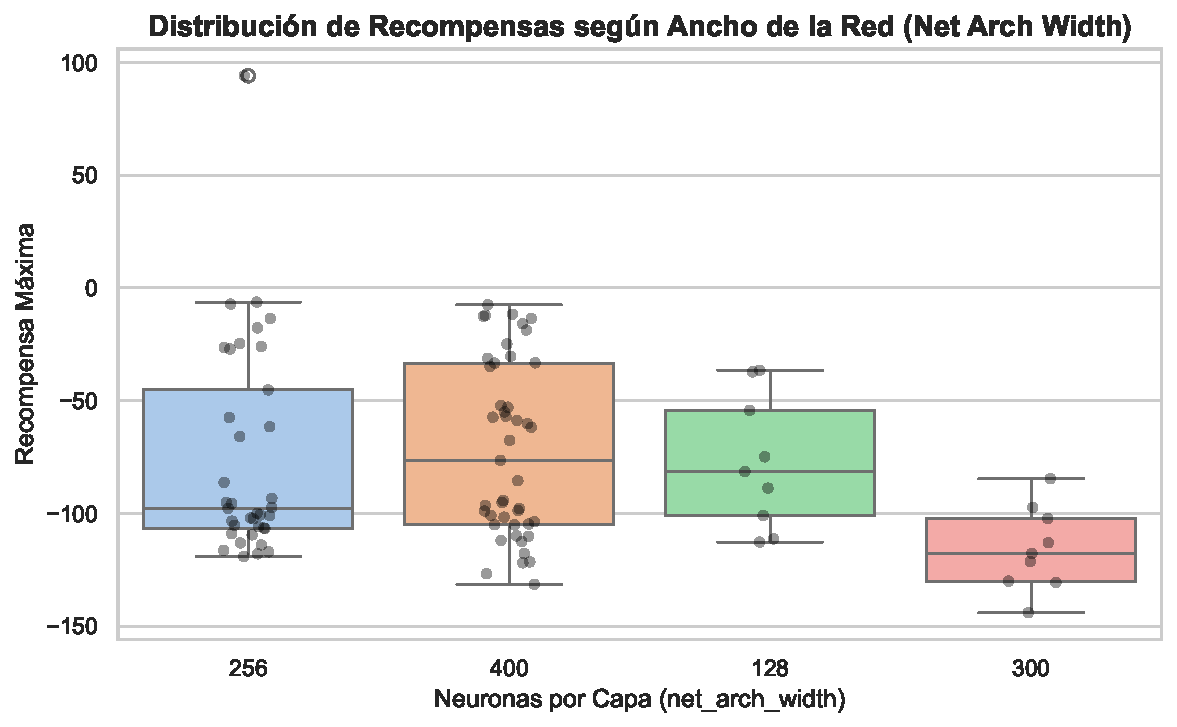
\includegraphics[width=\textwidth]{figuras/optuna_boxplot_arquitectura}
			\caption{Distribución de Recompensas según Ancho de la Red.}
			\label{fig:optunaboxplotarquitectura}
		\end{subfigure}
		\hfill
		% Subfigura (b)
		\begin{subfigure}[b]{0.48\textwidth}
			\centering
			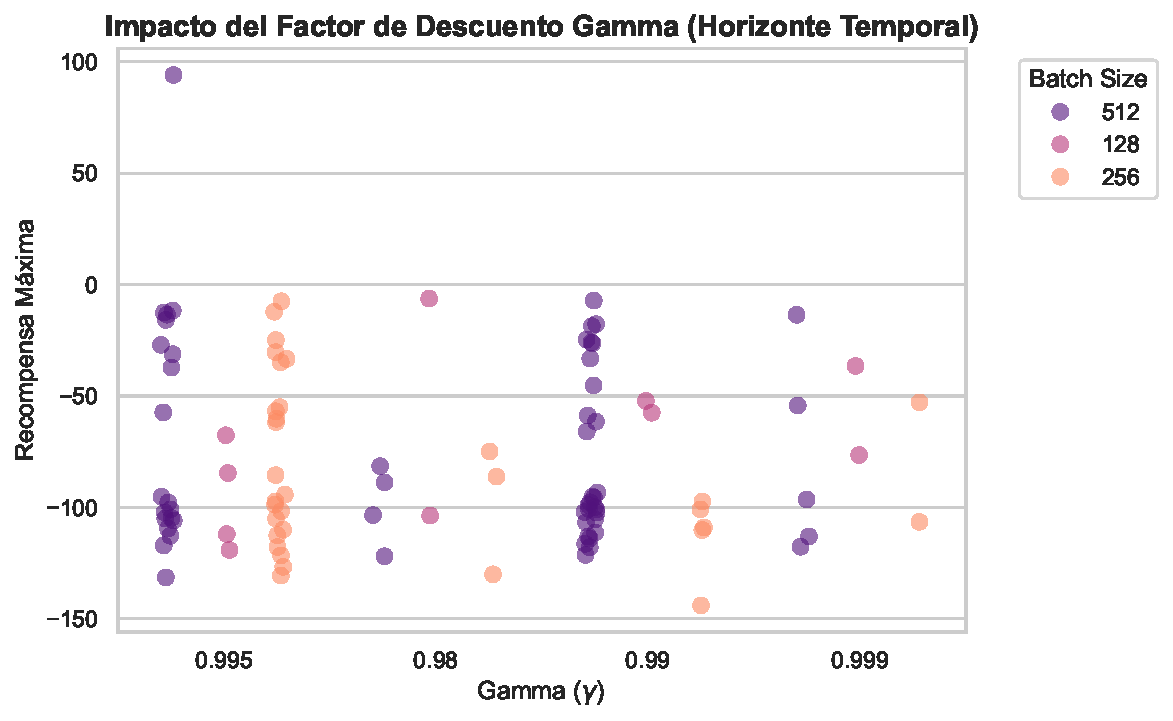
\includegraphics[width=\textwidth]{figuras/optuna_gamma_analysis}
			\caption{Impacto del Factor de Descuento $\gamma$.}
			\label{fig:optunagammaanalysis}
		\end{subfigure}
		
		\vspace{0.5cm} % Espacio vertical entre las filas
		
		% Subfigura (c)
		\begin{subfigure}[b]{0.48\textwidth}
			\centering
			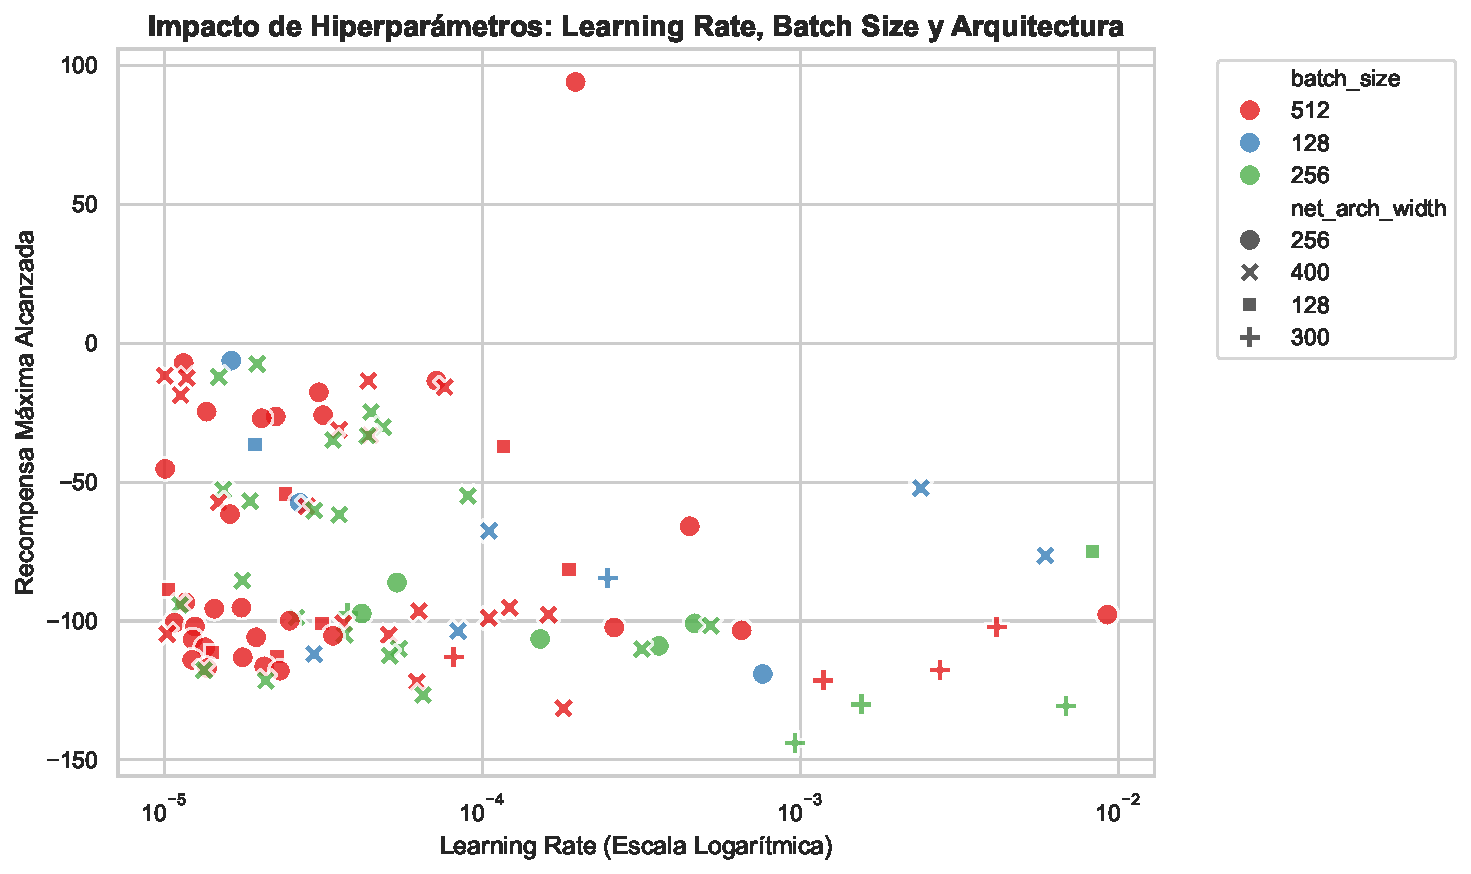
\includegraphics[width=\textwidth]{figuras/optuna_scatter_multidimensional}
			\caption{Sensibilidad del Parámetro Learning Rate.}
			\label{fig:optunascattermultidimensional}
		\end{subfigure}
		\hfill
		% Subfigura (d)
		\begin{subfigure}[b]{0.48\textwidth}
			\centering
			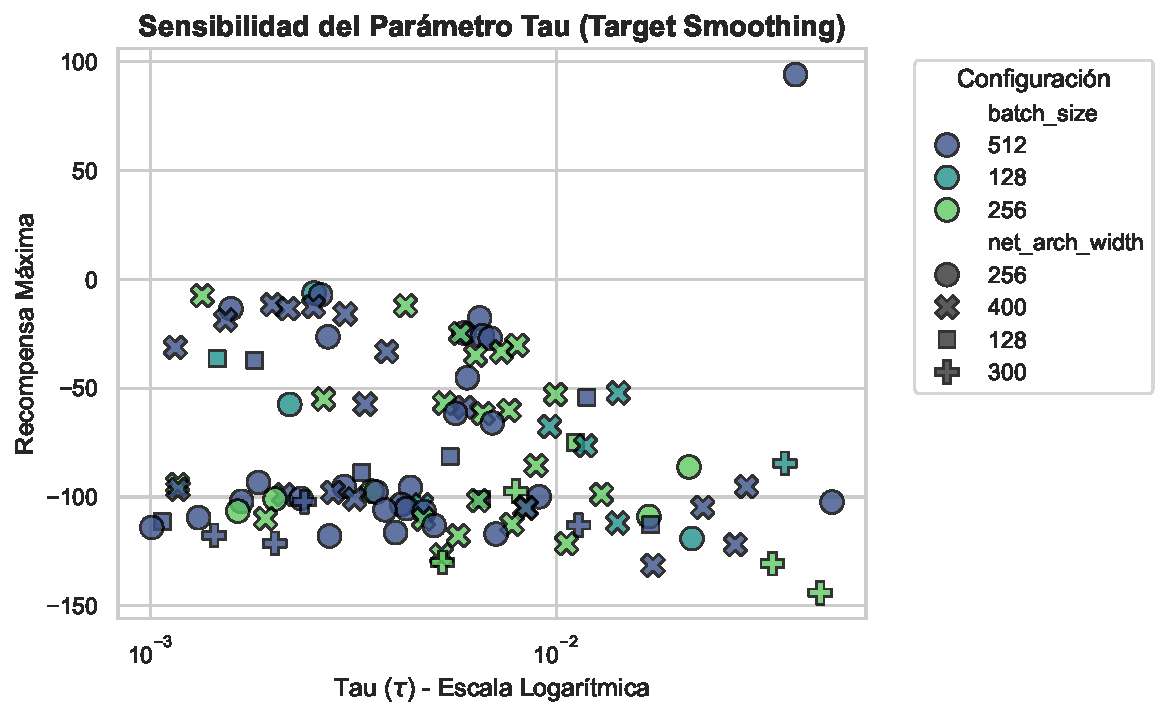
\includegraphics[width=\textwidth]{figuras/optuna_tau_analysis}
			\caption{Sensibilidad del Parámetro \(\tau\).}
			\label{fig:optunatauanalysis}
		\end{subfigure}
		
		\caption{Análisis de resultados de la optimización de hiperparámetros. Se evalúa el impacto de la arquitectura, el factor de descuento, la tasa de aprendizaje y el suavizado del objetivo en la recompensa máxima.}
		\label{fig:analisis_optuna_completo}
	\end{figure}
	
	Como se adelantó previamente, la evaluación temprana de hiperparámetros presenta limitaciones importantes. Las Figuras \ref{fig:graficorecompensatiempo} y \ref{fig:optunacurvastop5} muestran que el aprendizaje no es lineal donde la recompensa oscila durante los primeros miles de pasos hasta alcanzar un punto de inflexión donde mejora abruptamente. Por tanto, descartar modelos de forma prematura resulta problemático. De hecho, la Figura \ref{fig:optunacurvastop5} ilustra que, incluso entre las mejores configuraciones, el rendimiento inicial es inestable y no garantiza una tendencia.
	\newline
	
	Por otro lado, la Figura \ref{fig:graficorecompensatiempo} revela un comportamiento interesante ligado a la exploración del algoritmo. Incluso cuando el agente ya domina la tarea, se observan caídas puntuales en la recompensa. Esto ocurre porque el modelo sigue probando variaciones en sus movimientos para descubrir estrategias más óptimas. Asimismo, se detecta una fase intermedia donde la duración de los episodios es muy larga pero la recompensa no es máxima. Haciendo un símil humano, antes de aprender a correr de forma eficiente y directa, el agente primero debe aprender a estabilizarse para no caer y, posteriormente, a caminar con precaución. Esta progresión se corroborará más adelante en el análisis con un vídeo.
	\newline
	
	Finalmente, la Figura \ref{fig:graficotiempoepisodio} detalla la evolución del coste computacional. Al inicio del entrenamiento, el tiempo invertido por episodio es muy bajo porque el robot pierde el equilibrio casi al instante. Sin embargo, conforme aprende a mantenerse en pie, la duración de cada intento se estabiliza y el tiempo acumulado empieza a crecer de forma lineal. Aunque esta métrica no sirva para predecir el tiempo total de ejecución, proporciona un indicador indirecto para confirmar visualmente el momento exacto en el que el agente aprende a realizar la tarea.

\begin{figure}[H]
	\centering
	
	% Subfigura (a) - Fila superior, tamaño grande
	\begin{subfigure}[b]{0.6\textwidth}
		\centering
		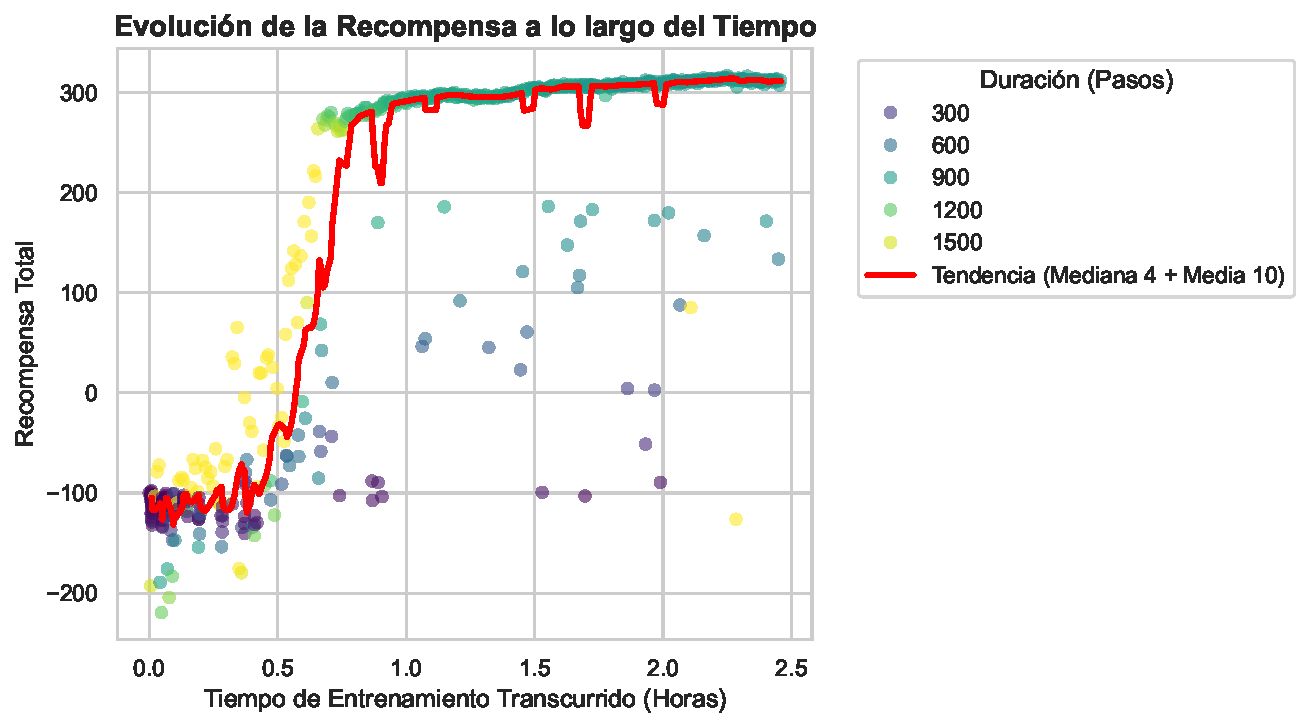
\includegraphics[width=\textwidth]{figuras/grafico_recompensa_tiempo}
		\caption{Evolución de la Recompensa a lo largo del Tiempo}
		\label{fig:graficorecompensatiempo}
	\end{subfigure}
	
	\vspace{0.6cm} % Espacio vertical entre la gráfica principal y las secundarias
	
	% Subfigura (b) - Fila inferior, izquierda
	\begin{subfigure}[b]{0.48\textwidth}
		\centering
		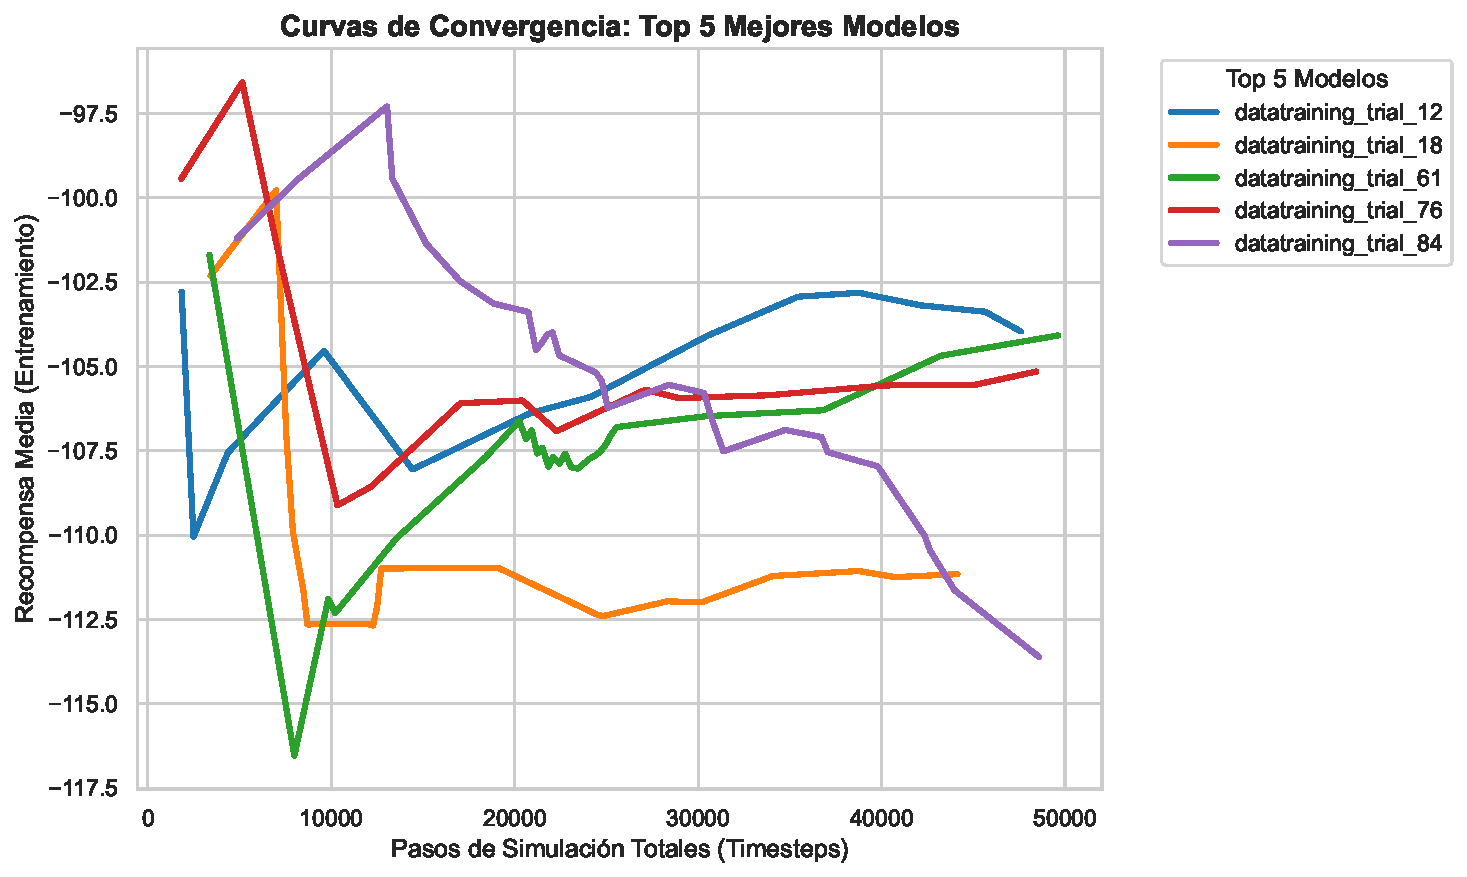
\includegraphics[width=\textwidth]{figuras/optuna_curvas_top5}
		\caption{Curvas de Convergencia: Top 5 Mejores Modelos}
		\label{fig:optunacurvastop5}
	\end{subfigure}
	\hfill
	% Subfigura (c) - Fila inferior, derecha
	\begin{subfigure}[b]{0.48\textwidth}
		\centering
		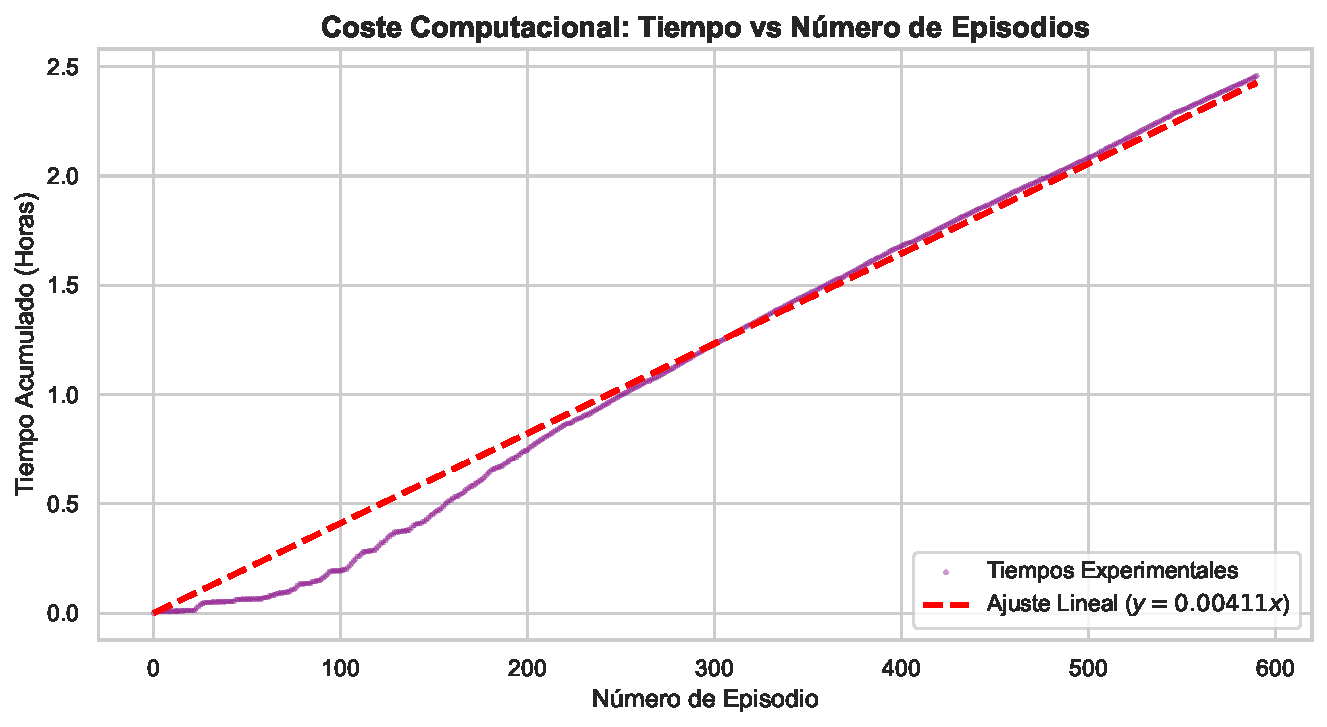
\includegraphics[width=\textwidth]{figuras/grafico_tiempo_episodio}
		\caption{Coste Computacional: Tiempo vs Número de Episodios}
		\label{fig:graficotiempoepisodio}
	\end{subfigure}
	
	\caption{Análisis temporal y de convergencia del entrenamiento. }
	\label{fig:analisis_tiempo_convergencia}
\end{figure}
	
La Figura \ref{fig:progreso_entrenamiento_final} presenta las métricas fundamentales que validan el éxito del entrenamiento del agente. En la subfigura (a), se aprecia cómo la recompensa de evaluación supera una fase inicial de alta inestabilidad para experimentar un crecimiento abrupto a partir de los 150,000 pasos, convergiendo finalmente hacia la meta de 300 puntos. Este dominio del entorno se corrobora con la subfigura (b), referida a la supervivencia del agente. Durante las primeras fases, el robot agota frecuentemente el límite máximo de la simulación (1600 pasos), lo que indica que sobrevive quedándose genuflexionado (como se ve en el vídeo). Sin embargo, una vez que la recompensa se maximiza, la duración de los episodios se reduce y se estabiliza en torno a los 800 pasos. Esto demuestra que el agente no solo ha aprendido a no caerse, sino que ha optimizado su locomoción para cruzar el terreno de la forma más rápida y directa posible.
\newline

Por otro lado, las subfiguras (c) y (d) ilustran la convergencia interna y la estabilidad matemática de las redes neuronales del algoritmo \textit{Soft Actor-Critic}. La pérdida del Actor (\textit{Actor Loss}) exhibe un comportamiento característico donde tras una fuerte fluctuación inicial provocada por la alta exploración y el ajuste dinámico de la entropía, la curva desciende de forma suave y monótona hasta alcanzar su estabilización. Simultáneamente, la pérdida del Crítico (\textit{Critic Loss}), representada en escala logarítmica, decrece drásticamente y establece un nivel base bajo. Aunque esta gráfica muestra picos de error constantes a lo largo de todo el entrenamiento, este ruido es normal, pues refleja los instantes en los que el agente experimenta con posturas nuevas o extrae transiciones inusuales de su memoria de repetición, obligando al Crítico a reajustar continuamente sus estimaciones de valor futuro.	
	
	
\begin{figure}[H]
	\centering
	% Subfigura (a)
	\begin{subfigure}[b]{0.48\textwidth}
		\centering
		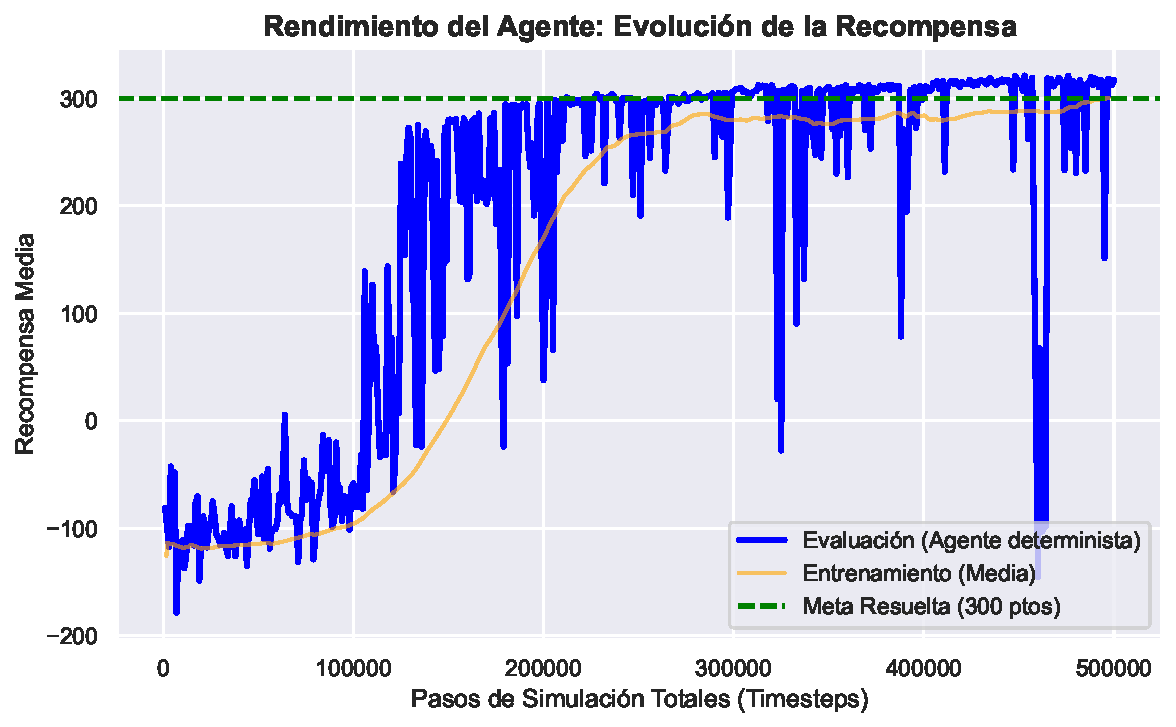
\includegraphics[width=\textwidth]{figuras/grafico_recompensas}
		\caption{Rendimiento del Agente: Evolución de la Recompensa}
		\label{fig:graficorecompensas}
	\end{subfigure}
	\hfill
	% Subfigura (b)
	\begin{subfigure}[b]{0.48\textwidth}
		\centering
		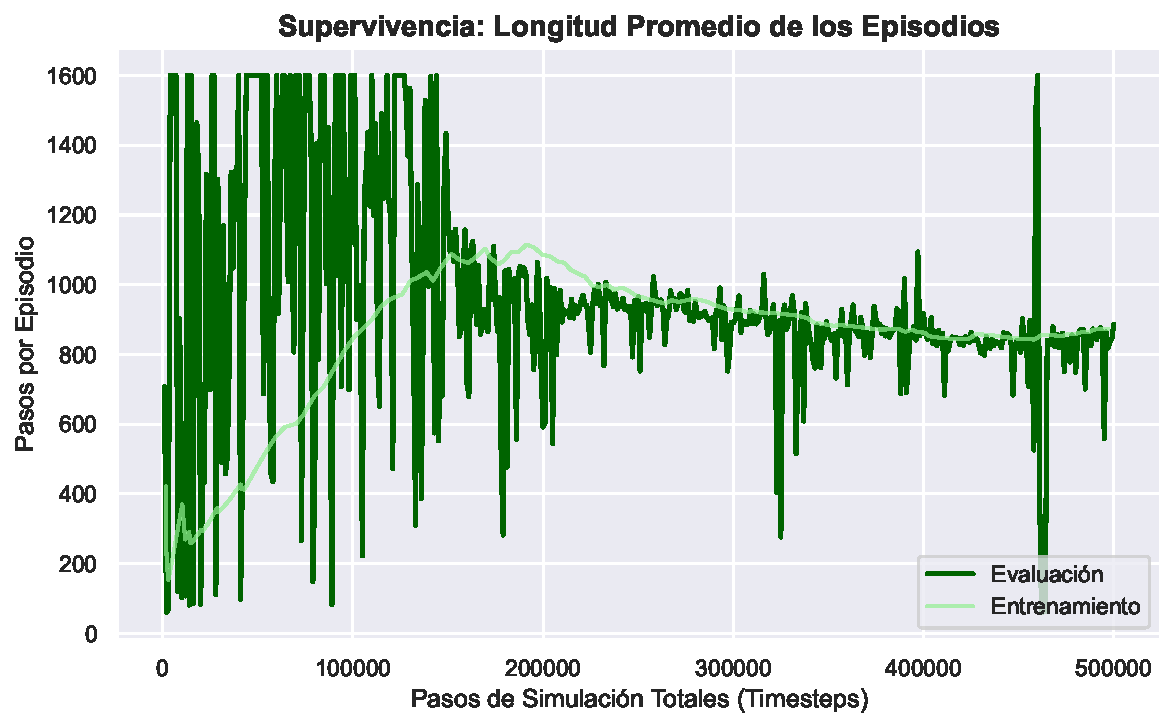
\includegraphics[width=\textwidth]{figuras/grafico_supervivencia}
		\caption{Supervivencia: Longitud Promedio de los Episodios}
		\label{fig:graficosupervivencia}
	\end{subfigure}
	
	\vspace{0.5cm} % Espacio vertical entre las filas
	
	% Subfigura (c)
	\begin{subfigure}[b]{0.48\textwidth}
		\centering
		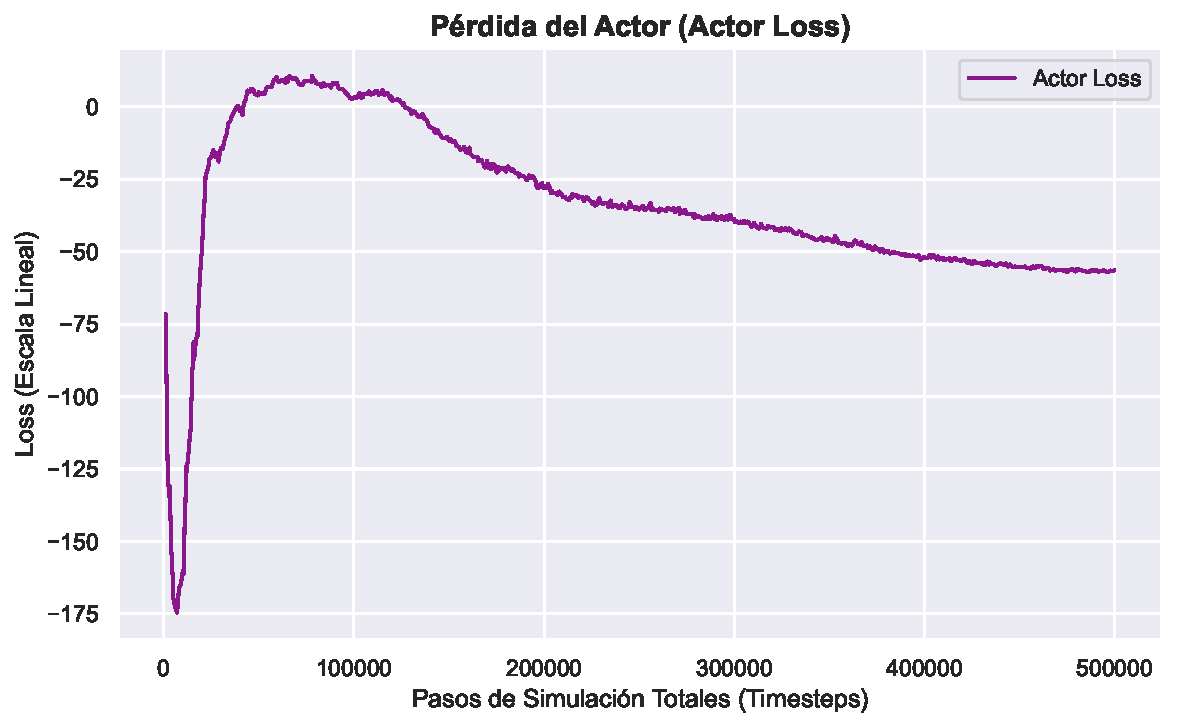
\includegraphics[width=\textwidth]{figuras/grafico_actor_loss}
		\caption{Pérdida del Actor (Actor Loss)}
		\label{fig:graficoactorloss}
	\end{subfigure}
	\hfill
	% Subfigura (d)
	\begin{subfigure}[b]{0.48\textwidth}
		\centering
		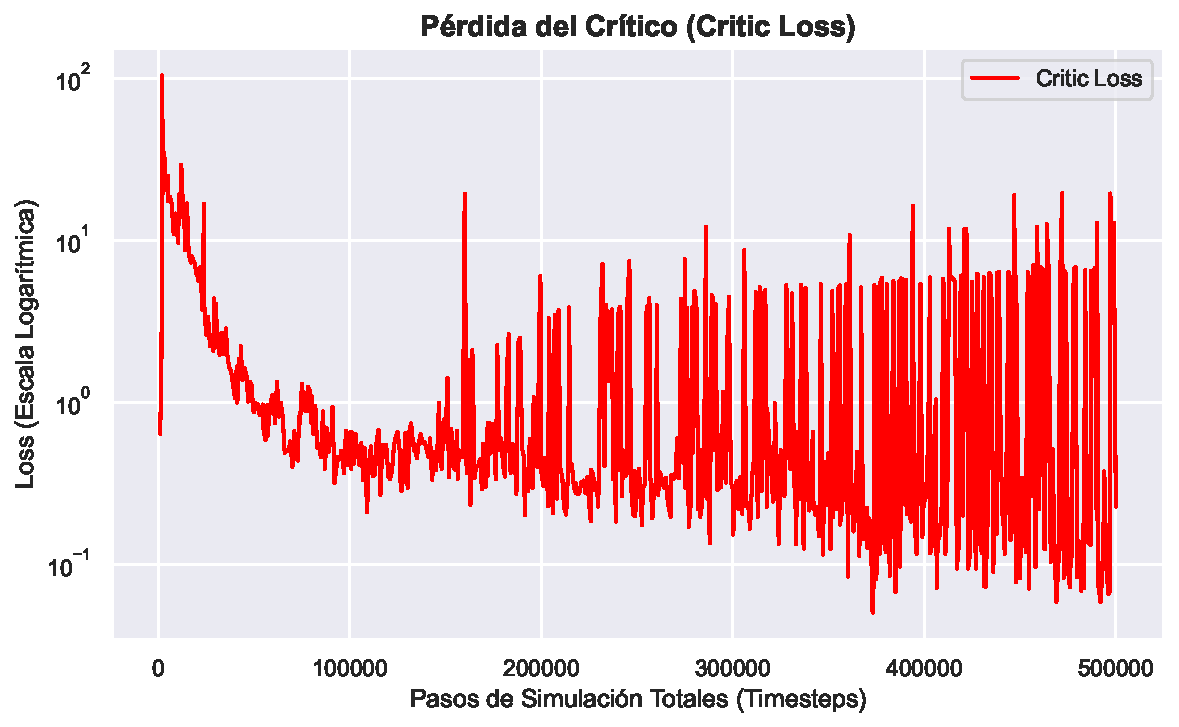
\includegraphics[width=\textwidth]{figuras/grafico_critic_loss}
		\caption{Pérdida del Crítico (Critic Loss)}
		\label{fig:graficocriticloss}
	\end{subfigure}
	
	\caption{Métricas de progreso durante el entrenamiento del agente final a lo largo de 500,000 pasos. Se observa la convergencia de la recompensa y la supervivencia.}
	\label{fig:progreso_entrenamiento_final}
\end{figure}
	
	Tras la optimización de hiperparámetros con \textit{optuna} y el entrenamiento final, se comprueba empíricamente que el agente aprende a andar de forma fluida\footnote{Vídeo demostrativo de la evolución del agente: \url{https://youtu.be/nI3171S9mWE}}.
	

	\section{Aspectos éticos en relación al problema}
	
	Aunque el entorno abordado en este proyecto se basa en una simulación bidimensional, el desarrollo de agentes autónomos mediante aprendizaje por refuerzo se puede extender al mundo real. La capacidad de enseñar a una máquina a caminar de forma autónoma, adaptándose al entorno sin reglas explícitas programadas a mano obliga a realizar una reflexión sobre su impacto ético y su alineación con los Objetivos de Desarrollo Sostenible (ODS) de la Agenda 2030 de las Naciones Unidas.
	
	\subsection{Alineación con los Objetivos de Desarrollo Sostenible (ODS)}
	
	El desarrollo de la robótica autónoma y los algoritmos de toma de decisiones impacta positivamente en varios objetivos globales:
	
	\begin{itemize}
		\item \textbf{ODS 3 (Salud y Bienestar):} Una de las transferencias tecnológicas más directas del problema del \textit{Bipedal Walker} es el campo de la biomecánica clínica en el diseño de prótesis robóticas inteligentes. Esto permitiría asistir a personas con discapacidades motoras o en procesos de rehabilitación, adaptando dinámicamente el paso del paciente a diferentes terrenos.
		\item \textbf{ODS 9 (Industria, Innovación e Infraestructura):} La optimización de algoritmos como \textit{Soft Actor Critic} impulsa la innovación tecnológica. El uso de robots bípedos permite el acceso en terrenos irregulares donde los vehículos con ruedas no pueden acceder, facilitando la automatización en la inspección de infraestructuras críticas, mantenimiento o logística.
		\item \textbf{ODS 8 (Trabajo Decente y Crecimiento Económico):} Los robots bípedos pueden ser desplegados en entornos de alto riesgo para los humanos, asumiendo las tareas peligrosas y promoviendo un entorno de trabajo más seguro.
	\end{itemize}
	
	\subsection{Consideraciones Éticas y Riesgos}
	
	A pesar de los beneficios potenciales, la aplicación empírica de este tipo de inteligencia artificial plantea dilemas éticos:
	
	\begin{itemize}
		\item \textbf{Dualidad de Uso:} La robótica con capacidad de desplazamiento todoterreno ha atraído tradicionalmente una gran inversión militar. Existe el riesgo ético de que algoritmos diseñados para la locomoción o el rescate sean adaptados para la creación de sistemas de armas autónomas letales. Como desarrolladores, es crucial abogar por regulaciones que limiten la automatización de la fuerza y prioricen fines civiles y pacíficos.
		\item \textbf{Impacto Medioambiental y ODS 13 (Acción por el Clima):} El entrenamiento de modelos, sumado a la búsqueda exhaustiva de hiperparámetros (\textit{Optuna}) realizada en este estudio, requiere un alto coste computacional. Este uso intensivo de procesamiento conlleva un consumo energético considerable y una huella de carbono asociada.
	\end{itemize}

	\newpage
	\bibliographystyle{ieeetr}
	\bibliography{bibliografia} 

		
\end{document}